\section{Results}
\label{sec:results}

\begin{table}[t]
\caption{Main comparison on the 112-case benchmark (Qwen2.5-7B-Instruct, $r=0.50$, seed
20261015). All arms of ours are constructed without access to the reference answer.
\emph{tokens} is the mean compressed-context length; \emph{leak} counts cases in which a
protected value is recoverable from question plus context. Arrows give the preferred
direction. $BCL$ $=$ \arm{budget\_cluster\_link}, $ABL$ $=$ \arm{alias\_budget\_link},
$ALB$ $=$ \arm{alias\_budget}, $BC$ $=$ \arm{budget\_cluster}. Controlled comparison is the
first three rows: compressing to $48.6\%$ of the original length costs $0.0109$ against the
no-compression aliasing arm, which is not significant. The uncompressed arm is the reference
value used to verify that a result set belongs to this benchmark.}
\label{tab:main}
\centering\small
\setlength{\tabcolsep}{3pt}
\begin{tabular}{lrrr}
\toprule
Arm & F1 $\uparrow$ & tokens $\downarrow$ & leak $\downarrow$ \\
\midrule
\arm{full}                 & 0.7189 & 7964 & 112/112 \\
\arm{alias}                & 0.6475 & 7824 & 0/112 \\
\textbf{\textsc{DARK}} & \textbf{0.6366} & \textbf{3869} & \textbf{0/112} \\
\arm{delete}               & 0.4916 & 7845 & 0/112 \\
BCL                        & 0.4308 & 3683 & 47/112 \\
ABL                        & 0.4219 & 3638 & 0/112 \\
ALB                        & 0.2232 & --- & 0/112 \\
BC                         & 0.2143 & --- & 8/112 \\
\bottomrule
\end{tabular}
\begin{tablenotes}\footnotesize
\item[] Paired differences against \textsc{DARK}: \arm{alias} $-0.0109$
$[-0.0824,+0.0612]$ (n.s.); \arm{full} $-0.0823$ $[-0.1610,-0.0041]$;
ABL $+0.2147$ $[+0.1224,+0.3085]$.
\end{tablenotes}
\end{table}


\subsection{Compression costs little}

Halving the prompt costs no measurable task quality. At an equal $50\%$ budget, aliasing the
whole context without compressing scores $0.6475$ and \textsc{DARK} scores $0.6366$ at
$48.6\%$ of the tokens. The paired difference is $-0.0109$ with a $95\%$ interval of
$[-0.0824,+0.0612]$, which does not exclude zero. Against not compressing and not sanitizing,
the deficit is $-0.0823$ $[-0.1610,-0.0041]$. That gap is the price of the privacy
constraint rather than of compression, since the aliasing arm pays it as well ($-0.0714$
against \arm{full}).

The comparison specific to our design is the lower block of the table. Two arms are
leak-free and compress to nearly the same length: \arm{alias\_budget\_link}, which aliases
globally and protects the anchor line, and \textsc{DARK}. The difference is $+0.2147$
$[+0.1224,+0.3085]$. The two do not differ in the privacy operation---both alias---but in
which region survives: one line, or the block containing it.

\begin{table*}[t]
\caption{Every arm on the same $2{,}728$ cases (Qwen2.5-7B-Instruct, $r=0.50$), with every
endpoint we measure. Published compressors are re-run through their reference implementations on
these cases; arms suffixed \arm{\_native} use each method's own default length. \emph{F1} and
\emph{EM} are the task metrics. \emph{GIC} is gold-in-context: the share of cases in which the
record carrying the reference answer survives compression at all, and it is the column that
separates the two families of method---every arm that keeps the anchor block holds it at $100\%$,
while the published compressors drop that record in $11$ to $54\%$ of cases. \emph{leak} is the
fraction of cases in which a protected value is recoverable from the prompt; \emph{tok} is the
mean realised context length. \textsc{DARK} is the only arm that reaches $100\%$ GIC and $0\%$
leakage together. Against the strongest leak-free published baseline, the masking wrapper, it
exceeds by $+0.3226$ $[+0.3050,+0.3413]$; against the strongest compressor, Quito-X, the
difference is $+0.0107$ $[-0.0091,+0.0304]$, i.e.\ not significant, at $0\%$ versus $98.1\%$
leakage. The \arm{lexcomp} row is from its own batch, where the control arms score $0.4934$ rather
than $0.4937$.}
\label{tab:external}
\centering\small
\setlength{\tabcolsep}{4pt}
\begin{tabular}{lllrrrrr}
\toprule
Method & Year & Family & F1 $\uparrow$ & EM $\uparrow$ & GIC $\uparrow$ & leak $\downarrow$ & tok \\
\midrule
\arm{full}                     & ---   & uncompressed         & 0.6081 & 0.5924 & 100.0\% & 100.0\% & 8482 \\
\arm{ext\_full}                & ---   & uncompressed (rerun) & 0.6078 & 0.5920 & 100.0\% & 100.0\% & 8482 \\
\textbf{\textsc{DARK}}         & ---   & ours (routes)        & \textbf{0.4937} & \textbf{0.4809} & \textbf{100.0\%} & \textbf{0.0\%} & 4146 \\
Quito-X                        & 2025  & query-aware          & 0.4831 & 0.4597 & 69.8\% & 98.1\% & 4242 \\
Quito-X \arm{\_native}         & 2025  & query-aware          & 0.4862 & 0.4630 & 69.7\% & 98.1\% & 4239 \\
CPC                            & 2025  & query-aware          & 0.4740 & 0.4600 & 82.7\% & 92.6\% & 4242 \\
CPC \arm{\_native}             & 2025  & query-aware          & 0.4523 & 0.4406 & 81.3\% & 93.4\% & 3855 \\
LongLLMLingua                  & 2024  & task-agnostic        & 0.4230 & 0.3893 & 70.3\% & 100.0\% & 4241 \\
Provence                       & 2025  & query-aware          & 0.4080 & 0.3985 & 88.9\% & 90.8\% & 4242 \\
Provence \arm{\_native}        & 2025  & query-aware          & 0.4047 & 0.3952 & 92.6\% & 88.8\% & 3995 \\
LexComp \arm{\_preprint}       & 2026  & lexical rules        & 0.3696 & 0.3299 & 65.0\% & 100.0\% & 5817 \\
\arm{alias\_budget\_link}      & ---   & ours, no key         & 0.3482 & 0.3398 & 57.6\% & 0.0\% & 3941 \\
\arm{budget\_cluster\_link}    & ---   & ours, anchor kept    & 0.3352 & 0.3270 & 57.6\% & 55.4\% & 3933 \\
\arm{quad4\_del}               & ---   & ours, delete         & 0.3142 & 0.3013 & 100.0\% & 0.0\% & 4147 \\
LLMLingua-2                    & 2024  & task-agnostic        & 0.2651 & 0.2386 & 62.6\% & 100.0\% & 4242 \\
Selective Context              & 2023  & task-agnostic        & 0.2588 & 0.2324 & 46.1\% & 100.0\% & 4055 \\
LLMLingua-2 \arm{\_native}     & 2024  & task-agnostic        & 0.2433 & 0.2181 & 59.8\% & 100.0\% & 4188 \\
\arm{mask\_llmlingua2}         & ---   & sanitize + compress  & 0.1712 & 0.1444 & 67.9\% & 0.0\% & 4242 \\
\arm{mask\_llmlingua2\_native} & ---   & sanitize + compress  & 0.1663 & 0.1397 & 67.5\% & 0.0\% & 4190 \\
\arm{alias\_budget}            & ---   & ours, global alias   & 0.1469 & 0.1455 & 47.5\% & 0.0\% & 3942 \\
\arm{budget\_cluster}          & ---   & ours, redundancy only & 0.0981 & 0.0968 & 47.5\% & 0.5\% & 3932 \\
\bottomrule
\end{tabular}
\end{table*}


\subsection{At scale, privacy is the only separation}

Table~\ref{tab:external} reports the $2{,}728$-case extension. \textsc{DARK} scores
$0.4937$, level with the strongest query-aware compressor (Quito-X, $0.4831$; difference
$+0.0107$, interval $[-0.0091,+0.0304]$) and above CPC ($0.4740$) and Provence ($0.4080$).
What separates the arms is leakage. Every published compressor leaves protected values in
the prompt, in $88.8\%$ to $100\%$ of cases, because concealing them is not among its
objectives. \textsc{DARK} leaves none. Among published baselines the only leak-free one is a
masking wrapper at $0.1712$, which \textsc{DARK} exceeds by $+0.3226$
$[+0.3050,+0.3413]$. The nearest arm of any kind that also leaks nothing is our own
global-alias ablation at $0.3482$, which \textsc{DARK} exceeds by $+0.1456$
$[+0.1253,+0.1662]$; those two arms differ only in which region survives, one line or the
block that contains it, so that margin is the routing rule and nothing else.

The GIC column of Table~\ref{tab:external} is worth a figure of its own, because it varies with
the source in a way the aggregate hides. Figure~\ref{fig:gic} breaks it out. The two arms that keep
the anchor block are flat at $100\%$ on all six sources. Every published compressor is a patchwork:
Quito-X retains the record in $17\%$ of \arm{privacylens} cases and $100\%$ of \arm{simuhome} ones,
Selective Context in $3\%$ of \arm{simuhome} and $100\%$ of \arm{smartbench\_tdcs}. A rule tuned on
one corpus and reported on another would move by tens of points without its F1 budget changing.

The same figure is the reason we do not treat GIC as the headline: the delete variant is equally
flat. Keeping the block is what determines the column, and the operation is invisible to it. That
is the separation Table~\ref{tab:ri} exists to make.

\begin{figure*}[t]
\centering
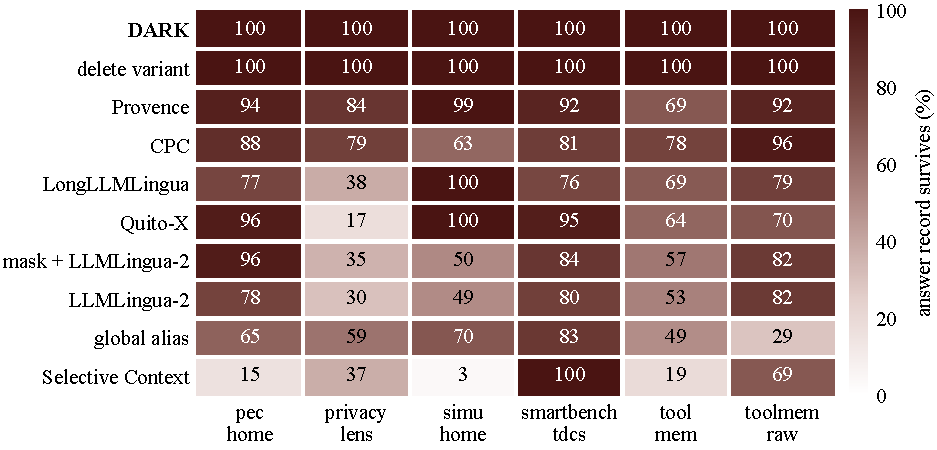
\includegraphics[width=\textwidth]{figures/fig_gic.pdf}
\caption{Gold-in-context by arm and source: the share of cases in which the record carrying the
reference answer survives compression at all. Darker is higher. The two arms that keep the anchor
block are flat at $100\%$ across six corpora; every published compressor is patchwork, and some
cells are near zero---Selective Context retains the answer record in $3\%$ of \arm{simuhome} cases,
Quito-X in $17\%$ of \arm{privacylens} cases. A number reported on one corpus would not transfer to
another. The figure also shows why GIC alone does not justify our design: the delete variant is as
flat as \textsc{DARK}, so this column measures the surviving region and says nothing about the
operation applied inside it. Table~\ref{tab:ri} makes that second distinction.}
\label{fig:gic}
\end{figure*}

Figure~\ref{fig:frontier} puts the same numbers on both axes at once, and attaches an interval
to each of them, because a point estimate in the corner of a plot invites the reading that the
axes were chosen after the fact. Panel~(a) is the frontier: \textsc{DARK} sits alone in the
upper-left, and the interval on its leakage is $[0,0.14]\%$ rather than a bare zero. Panel~(b) is
the part that keeps the figure honest. Paired against each comparator on the same cases,
\textsc{DARK} is ahead of every arm that leaks nothing by at least $0.14$ F1, and ahead of
Provence and LongLLMLingua by $0.086$ and $0.071$---all intervals clearing zero. Against
Quito-X ($+0.0107$, $[-0.0091,+0.0304]$) and CPC ($+0.0198$, $[-0.0008,+0.0397]$) the interval
contains zero, and we report those two rows as unresolved rather than as a win. That is the
whole claim: on F1 this experiment does not separate us from the best compressor, and on leakage
it separates us from every one of them.

\subsection{Which half the aggregate hides}
\label{sec:regimes}

\begin{table*}[t]
\caption{The same arms as Table~\ref{tab:external}, split by whether the question names a
protected value. A \emph{multi-entity} question names an account that is itself a protected value;
a \emph{needle} question names a record identifier that is not. $\Delta$ is the paired difference
\textsc{DARK} minus that row's method on the same cases, with a $95\%$ percentile bootstrap interval
over $4{,}000$ resamples (seed 7); positive means \textsc{DARK} is ahead, and a blank cell is the
\textsc{DARK} row itself. Leakage is recomputed inside each half. The aggregate in
Table~\ref{tab:external} averages these two columns, and they move in opposite directions.}
\label{tab:split}
\centering\footnotesize
\setlength{\tabcolsep}{4pt}
\begin{tabular}{lrrrrrr}
\toprule
 & \multicolumn{2}{c}{multi-entity ($n=1{,}500$)} & \multicolumn{2}{c}{needle ($n=1{,}228$)} & \multicolumn{2}{c}{$\Delta$ vs \textsc{DARK}} \\
\cmidrule(lr){2-3}\cmidrule(lr){4-5}\cmidrule(lr){6-7}
Method & F1 $\uparrow$ & leak $\downarrow$ & F1 $\uparrow$ & leak $\downarrow$ & multi & needle \\
\midrule
\arm{full} & 0.5485 & 100.0\% & 0.6810 & 100.0\% & $\mathbf{-0.221}$ {\scriptsize$[-0.248,-0.195]$} & $+0.016$ {\scriptsize$[-0.003,+0.035]$} \\
\textbf{\textsc{DARK}} & 0.3273 & 0.0\% & 0.6970 & 0.0\% & --- & --- \\
Quito-X & 0.4587 & 100.0\% & 0.5129 & 95.7\% & $\mathbf{-0.131}$ {\scriptsize$[-0.159,-0.105]$} & $\mathbf{+0.184}$ {\scriptsize$[+0.156,+0.212]$} \\
CPC & 0.3893 & 100.0\% & 0.5775 & 83.6\% & $\mathbf{-0.062}$ {\scriptsize$[-0.093,-0.031]$} & $\mathbf{+0.120}$ {\scriptsize$[+0.094,+0.145]$} \\
LongLLMLingua & 0.4083 & 100.0\% & 0.4409 & 100.0\% & $\mathbf{-0.081}$ {\scriptsize$[-0.110,-0.053]$} & $\mathbf{+0.256}$ {\scriptsize$[+0.229,+0.284]$} \\
Provence & 0.3503 & 89.5\% & 0.4783 & 92.4\% & $-0.023$ {\scriptsize$[-0.054,+0.007]$} & $\mathbf{+0.219}$ {\scriptsize$[+0.192,+0.247]$} \\
LexComp \arm{\_preprint} & 0.4044 & 100.0\% & 0.3270 & 100.0\% & $\mathbf{-0.077}$ {\scriptsize$[-0.107,-0.048]$} & $\mathbf{+0.370}$ {\scriptsize$[+0.341,+0.401]$} \\
\arm{quad4\_del} & 0.0000 & 0.0\% & 0.6980 & 0.0\% & $\mathbf{+0.327}$ {\scriptsize$[+0.305,+0.351]$} & $-0.001$ {\scriptsize$[-0.011,+0.008]$} \\
LLMLingua-2 & 0.2552 & 100.0\% & 0.2772 & 100.0\% & $\mathbf{+0.072}$ {\scriptsize$[+0.041,+0.101]$} & $\mathbf{+0.420}$ {\scriptsize$[+0.391,+0.447]$} \\
\arm{mask\_llmlingua2} & 0.0000 & 0.0\% & 0.3803 & 0.0\% & $\mathbf{+0.327}$ {\scriptsize$[+0.305,+0.351]$} & $\mathbf{+0.317}$ {\scriptsize$[+0.289,+0.344]$} \\
\arm{alias\_budget} & 0.0907 & 0.0\% & 0.2155 & 0.0\% & $\mathbf{+0.237}$ {\scriptsize$[+0.210,+0.263]$} & $\mathbf{+0.482}$ {\scriptsize$[+0.453,+0.511]$} \\
\arm{budget\_cluster} & 0.0007 & 0.2\% & 0.2171 & 0.9\% & $\mathbf{+0.327}$ {\scriptsize$[+0.304,+0.350]$} & $\mathbf{+0.480}$ {\scriptsize$[+0.452,+0.510]$} \\
\bottomrule
\end{tabular}
\end{table*}



\begin{figure}[t]
\centering
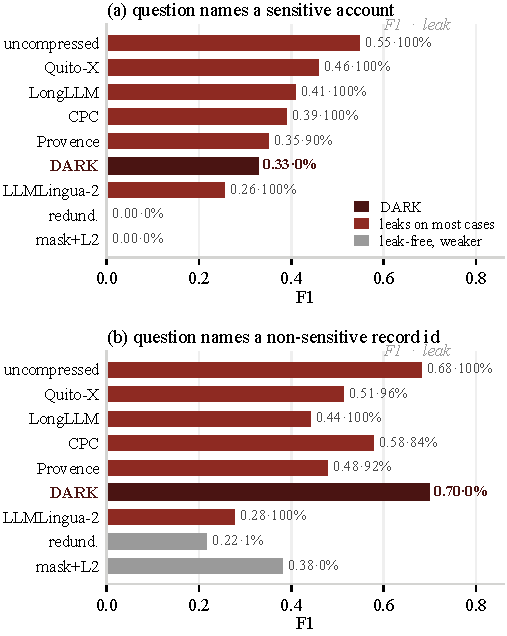
\includegraphics[width=\columnwidth]{figures/fig_regimes.pdf}
\caption{The same comparison, split by whether the question names a protected value. Bars are F1,
and the number after each bar is F1 followed by the share of cases in which a protected value is
recoverable from the prompt. (a)~When the question names a sensitive account, the arms above us on
F1 are exactly the arms that leak on $89.5$--$100\%$ of these cases, and the only leak-free arms that
answer at all are ours. (b)~When the question names a record identifier that carries no protected
value, aliasing is unnecessary, the cost disappears, and \textsc{DARK} leads every compressor.
Panel~(a) is the honest cost of the design and panel~(b) is where it is free; both come from the
same rule, applied without a flag that says which regime it is in.}
\label{fig:regimes}
\end{figure}


The headline comparison is a tie, $0.4937$ against $0.4831$ over all $2{,}728$ cases. That tie
averages two populations that move in opposite directions, and the split between them is not a
reporting convenience: it is the distinction the paper is about. When the question names a
sensitive account, the reader has to resolve an invented token before it can answer, and that
resolution costs F1. When the question names a record identifier that carries no protected value,
there is nothing to alias and the cost does not arise.

Table~\ref{tab:split} and Figure~\ref{fig:regimes} separate the two. On the $1{,}500$ multi-entity
cases, every compressor that beats us on F1 leaks on $89.5$--$100\%$ of those same cases: Quito-X
gains $+0.1314$ over us and forwards a protected value in all $1{,}500$, and the uncompressed
prompt gains $+0.2212$. Among the arms that leak nothing we are
the only one that answers at all, at $0.3273$ against $0.0007$ for the next leak-free arm, a gap of
$+0.3267$ $[+0.3040,+0.3500]$. On the $1{,}228$ needle cases the order reverses, and it reverses
against every arm in the table: we lead the two strongest compressors by $+0.1842$
$[+0.1558,+0.2124]$ and $+0.1196$ $[+0.0943,+0.1451]$, the 2026 rule-based compressor by $+0.3699$,
LLMLingua-2 by $+0.4198$, and we match the uncompressed prompt ($+0.0160$ $[-0.0032,+0.0348]$) at
half its length.

One mechanism produces both halves. The F1 cost is what it takes to make the referent unreadable,
so it is paid exactly where the referent is the secret and nowhere else. The aggregate tie is
therefore not a compromise between two mediocre outcomes: it is a large loss in one regime and a
large win in the other, and only one of those regimes involves a choice. Where the anchor is not
sensitive, leaking buys nothing, and the compressors pay it anyway.


\begin{figure*}[t]
\centering
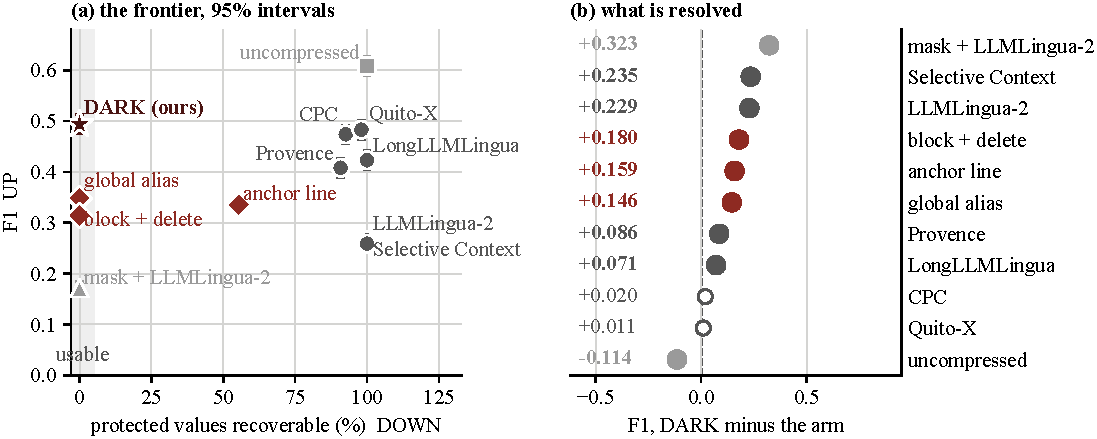
\includegraphics[width=\textwidth]{figures/fig_frontier.pdf}
\caption{Where each arm sits, and which of the differences the experiment resolves. (a)~Every
arm run at $2{,}728$ cases, with a $95\%$ interval on both coordinates. F1 uses a percentile
bootstrap over cases. Leakage is a proportion and several arms sit at exactly $0\%$ or $100\%$,
where the bootstrap is degenerate, so it uses a Wilson score interval instead; an arm that leaks
nothing in $2{,}728$ cases then has an upper bound of $0.14\%$, which is what a measured zero
looks like. Markers are coloured by provenance: grey for the uncompressed reference and the
published compressors, dark red for ablations of our own design, black for the full rule.
(b)~\textsc{DARK} minus each comparator, paired on the same cases, with a $95\%$ bootstrap
interval; a filled marker has an interval that excludes zero and a hollow one does not.
The two hollow rows are the load-bearing ones: against Quito-X and CPC the interval contains
zero, so we call those differences unresolved.}
\label{fig:frontier}
\end{figure*}

The table also carries a 2026 rule-based compressor, run on CPU at its most aggressive preset~\cite{chokshi-lexical-2026}. It realises $5{,}817$ context tokens---more than we spend---scores $0.3696$, and leaks in $100\%$ of cases. Section~\ref{sec:analysis} isolates why: its rules delete the braces and rename the keys that make a record a record.

The aggregate also hides a split, which Section~\ref{sec:regimes} and
Table~\ref{tab:split} take up: the two halves move in opposite directions.

The reading we take from this table is narrow. A query-aware compressor reaches the same F1
as our rule at the same budget, but only by forwarding the value the question names. When
that value must not be forwarded, the compressor loses the task, as the masking row shows,
and the routing rule does not.

Figure~\ref{fig:persource} qualifies the aggregate: the $0.4937$ is not uniform across
sources. Deleting the anchor unit instead of aliasing it costs almost nothing on
\texttt{privacylens} ($0.467$ against $0.437$) and collapses \texttt{simuhome} ($0.619$
against $0.029$) and \texttt{pec\_home} ($0.676$ against $0.274$). A mean over six sources
is what makes that look like one effect. \textsc{DARK} sits below the uncompressed arm
everywhere but is the arm closest to it on four of six sources; on \texttt{smartbench\_tdcs}
the anchor-protecting arm is closer, and on \texttt{toolmem} all four arms fall within
$0.04$ of each other. On \texttt{toolmem\_raw} every arm is below $0.45$, so the source
rather than the operation is the bottleneck. The privacy rows are the part that does not
vary: the uncompressed prompt exposes a protected value in $100\%$ of cases on every source,
\textsc{DARK} and the delete variant in none, and the anchor-protecting arm leaks in five of
six because protecting the block keeps the neighbouring units that carry the value.

\begin{figure*}[t]
\centering
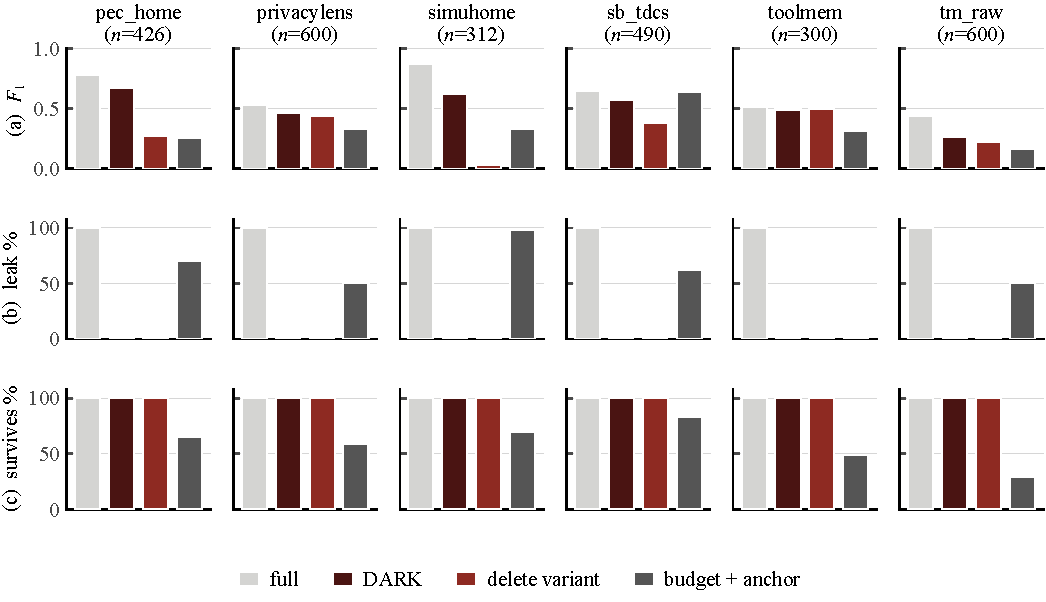
\includegraphics[width=\textwidth]{figures/fig_persource.pdf}
\caption{Per-source behaviour on the $2{,}728$-case extension at $r=0.50$, one panel per
source and one row per metric; $n$ under each column is the number of cases.
(a)~\textsc{DARK} sits below the uncompressed arm everywhere and is the closest arm to it on
four of six sources, but the two effects that matter are local: on \texttt{simuhome} the
delete variant falls to $0.029$ against \textsc{DARK}'s $0.619$, and on \texttt{toolmem\_raw}
all arms are below $0.45$ because the answers themselves are hard. (b)~Leakage does not vary
by source: the uncompressed arm exposes a protected value in every case, while \textsc{DARK}
and the delete variant expose none on any source---a bar of zero height is a zero, not
missing data---and the anchor-protecting arm leaks in five of six. (c)~The answer-bearing record survives in $100\%$ of cases for
the uncompressed arm, \textsc{DARK} and the delete variant, and in $29$--$83\%$ for the
anchor-protecting arm; the whole-vs-line distinction of Figure~\ref{fig:pipeline}(c) is what
separates those three from the fourth.}
\label{fig:persource}
\end{figure*}

\begin{table}[t]
\caption{Budget curve on the 112-case benchmark. Every row satisfies its budget with zero
overshoot. \textsc{DARK} is the strongest budget arm at all five ratios; its advantage
narrows as the budget grows, and its own score peaks at $r=0.50$ because at $r=0.75$ the
additional refill text is noise. The last row gives the mean realised context length in tokens.}
\label{tab:budget}
\centering\small
\setlength{\tabcolsep}{3pt}
\resizebox{\columnwidth}{!}{%
\begin{tabular}{lrrrrr}
\toprule
Arm & @0.10 & @0.15 & @0.25 & @0.50 & @0.75 \\
\midrule
\textbf{\textsc{DARK}} & \textbf{0.4357} & \textbf{0.4681} & \textbf{0.5116} & \textbf{0.6366} & \textbf{0.6158} \\
\arm{quad4\_del}           & 0.3297 & 0.3788 & 0.3955 & 0.5205 & 0.5086 \\
BCL                        & 0.2304 & 0.2052 & 0.2310 & 0.4308 & 0.5576 \\
ABL                        & 0.2304 & 0.2052 & 0.2488 & 0.4219 & 0.5512 \\
\midrule
realised tokens            & 656 & 1033 & 1913 & 3869 & 5830 \\
\bottomrule
\end{tabular}}
\vspace{2pt}
{\footnotesize Uncompressed reference: F1 $0.7189$ at $7964$ tokens.}
\end{table}


\begin{figure*}[t]
\centering
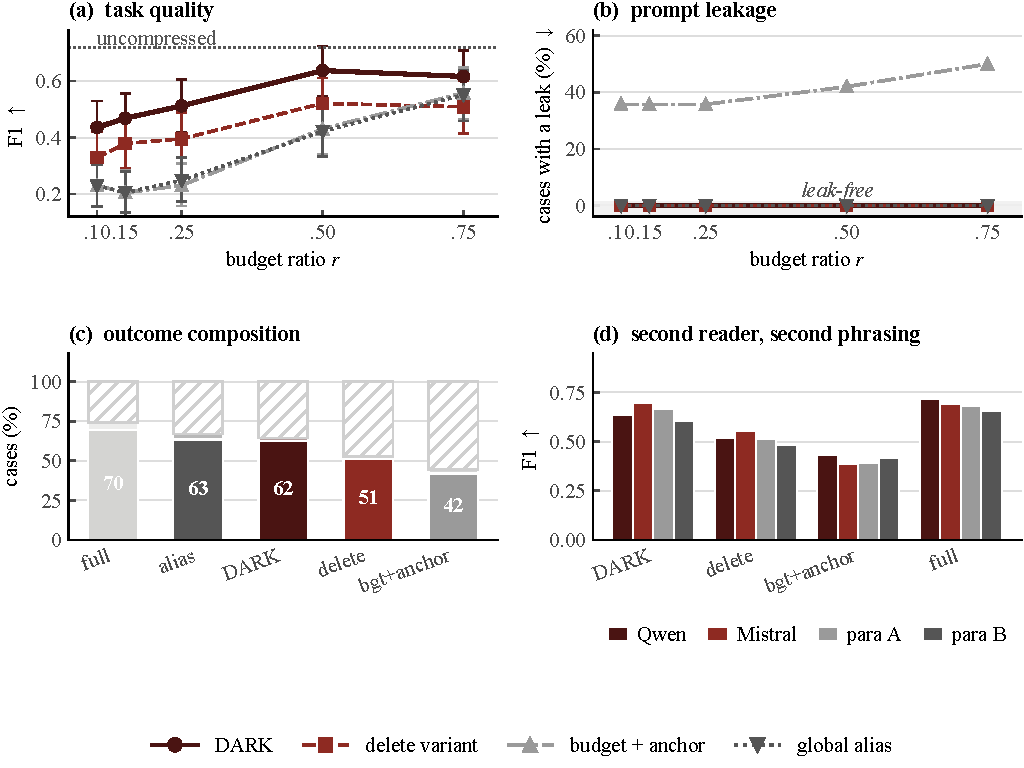
\includegraphics[width=\textwidth]{figures/fig1_main.pdf}
\caption{Behaviour across the budget sweep on the 112-case benchmark; the same property at full
scale, with the published compressors on it, is Figure~\ref{fig:budgetall}. (a) F1 at five ratios
with bootstrap $95\%$ intervals over cases; the dotted line is the uncompressed reference. (b) Fraction of
cases in which a protected value is recoverable from the prompt. \textsc{DARK}, the
delete variant and the global-alias arm stay at zero for the whole range, while the arm that
compresses raw text leaks in $35.7\%$ of cases at tight budgets and $50.0\%$ at $r=0.75$, so
its apparent parity at loose budgets is bought with exposure. (c) Composition of case
outcomes at $r=0.50$: solid is an exact answer, the pale band is a partial match, hatched is
a wrong or \textsc{unknown} answer. (d) The same four arms at $r=0.50$ under the original
reader, a second reader, and two mechanical rewritings of the question. \textsc{DARK} is the
only arm that gains from the reader change ($0.6366\to0.6946$) and draws level with the
uncompressed arm there ($0.6931$); under both rewritings the ordering of the four arms is
unchanged.}
\label{fig:budget}
\end{figure*}

\subsection{Other readers, other phrasings}

On Mistral-7B-Instruct-v0.3 at $r=0.50$, \textsc{DARK} scores $0.6946$ against $0.6366$
on Qwen2.5-7B. Every other arm loses ground when the reader changes: \arm{full} $-0.0258$,
\arm{alias} $-0.0544$, \arm{delete} $-0.0357$, \arm{alias\_budget\_link} $-0.0471$,
\arm{budget\_cluster\_link} $-0.0471$. The routing rule is the only arm that improves, which
is consistent with the mechanism: a second reader gains more from a cleaned, budgeted prompt
than from a long one.

Against two mechanical rewritings of the question, \textsc{DARK} scores $0.6637$ and
$0.6023$ against $0.6366$ on the original, a maximum change of $-0.0343$. The uncompressed
arm changes by $-0.0614$ over the same rewritings. The margin over
\arm{alias\_budget\_link} remains significant in all three conditions ($+0.2147$, $+0.2711$,
$+0.1994$). The check is relevant because the rule keys on a mention of the queried entity,
and a rewriting could in principle disturb that mention; in these variants it does not.

\begin{table}[t]
\caption{Two readers, same $2{,}728$ cases, same prompts. The quantity of interest is not the
absolute F1---the readers differ in it---but the \emph{cost} of the rule, the paired difference
between \textsc{DARK} and the uncompressed arm on identical inputs. That cost is
$-0.1144$ on the first reader and $-0.1118$ on the second, and the difference between the two
costs is $+0.0026$ with an interval that contains zero. We report that as ``the two readers were
not distinguished on this quantity'', not as a demonstration that the cost is equal: an interval
containing zero bounds what this experiment can claim, and a non-inferiority statement would
need a margin fixed in advance.}
\label{tab:crossreader}
\centering\small
\setlength{\tabcolsep}{4pt}
\resizebox{\columnwidth}{!}{%
\begin{tabular}{lrrrrr}
\toprule
Reader & $n$ & full F1 & \textsc{DARK} F1 & \textsc{DARK}$-$full [95\% CI] & leak \\
\midrule
Qwen2.5-7B-Instruct      & 2{,}728 & 0.6081 & 0.4937 & $-0.1144$ $[-0.1326,-0.0971]$ & $0\%$ \\
Granite-3.1-8B-Instruct  & 2{,}728 & 0.5764 & 0.4647 & $-0.1118$ $[-0.1293,-0.0941]$ & $0\%$ \\
\midrule
difference of the costs  &         &        &        & $+0.0026$ $[-0.0201,+0.0245]$ & \\
\bottomrule
\end{tabular}}
\end{table}


\paragraph{The cost of the rule does not depend on the reader.}
Table~\ref{tab:crossreader} repeats the comparison on a second reader from a different family.
The two readers do not agree on absolute F1---Granite is $0.03$ below Qwen on the uncompressed
arm---so the absolute numbers cannot be pooled. The quantity that does carry over is the
\emph{cost} of the rule: on identical inputs, \textsc{DARK} gives up $0.1144$ on the first reader
and $0.1118$ on the second. The difference between those two costs is $+0.0026$
$[-0.0197,+0.0249]$, which does not exclude zero, and we report it that way. What the experiment
supports is that the mechanism is not tuned to one tokenizer or one instruction set: it is the
same construction, the same prompts and the same cost, on a reader trained by a different
organisation. What it does not support is a claim about readers larger than the two tested; we
say so again in Section~\ref{sec:discussion}.

\begin{figure*}[t]
\centering
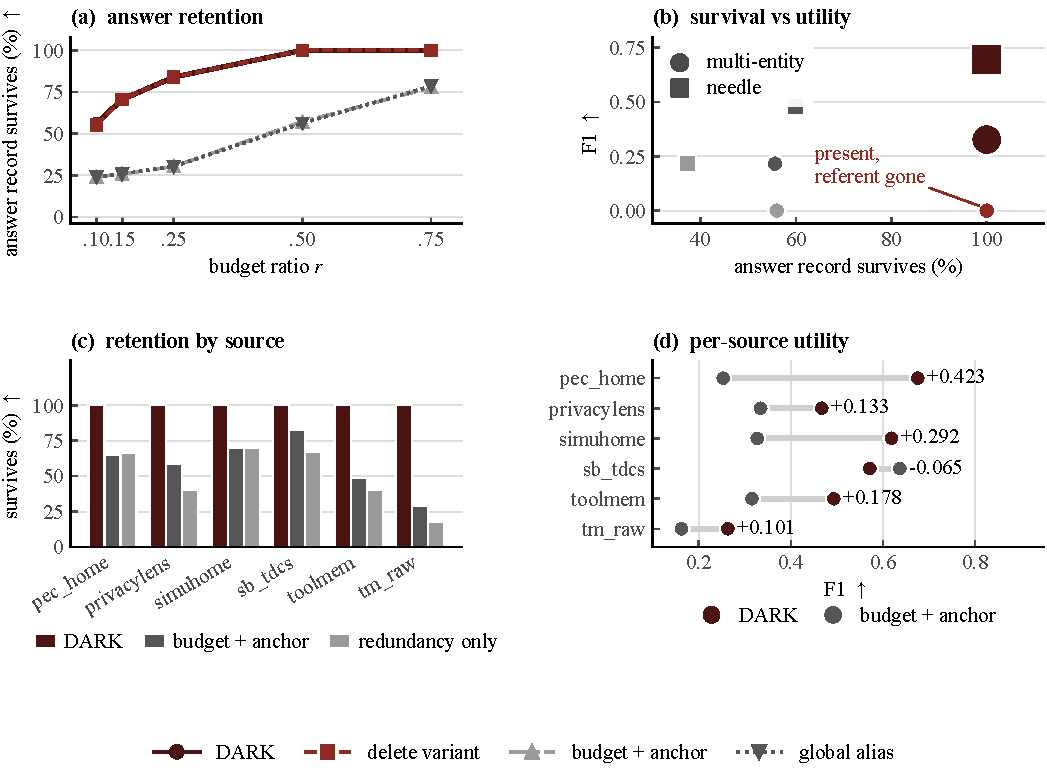
\includegraphics[width=\textwidth]{figures/fig2_diagnostic.pdf}
\caption{Answer retention and what it does not explain. (a) Fraction of the 112 benchmark
cases in which the record carrying the reference answer survives compression, as the budget
varies. \textsc{DARK} and the delete variant coincide almost exactly: the
alias-instead-of-delete rule does not change \emph{which} units survive. (b) Survival against
F1 on the $2{,}728$-case extension; circles are multi-entity cases and squares are needle
cases, and the four arms are the redundancy-only rule, the same rule with the anchor line
protected, \textsc{DARK}, and the delete variant. The delete variant sits at $100\%$ survival
and $0.0000$ F1 on multi-entity cases: the information is in the prompt and cannot be
located. (c) Retention within each source at
$r=0.50$. (d) Per-source F1, \textsc{DARK} against the anchor-protected arm, with the
paired difference printed at each row.}
\label{fig:survival}
\end{figure*}

\subsection{What protection costs, measured against budget}
\label{sec:budgetall}

A budget sweep holds the corpus and the reader fixed and varies only how much of the prompt
survives, so it is the one experiment that can price referential integrity. Figure~\ref{fig:budgetall}
runs it on all $2{,}728$ cases at four ratios with two redundancy arms as brackets: one prunes and
protects nothing, the other adds exactly one thing---it keeps the anchor line verbatim.

\textsc{DARK} is the only arm that improves as the budget grows without ever leaking. It scores
$0.3297$ at $5\%$, $0.3635$ at $10\%$, $0.4168$ at $15\%$ and $0.4937$ at $50\%$, at $0\%$ measured
leakage at every point. Against pruning alone it leads by $+0.092$, $+0.089$, $+0.145$ and $+0.158$
across the same four ratios, which is what the routing rule is worth when nothing is forwarded.

The arm that keeps the anchor verbatim scores higher only where it can afford to forward the value.
It peaks at $0.6241$ at $r=0.15$, ahead of \textsc{DARK}, and its leakage at that point is $39\%$;
at $r=0.05$ it forwards a protected value in $21\%$ of cases and at $r=0.50$ in $55\%$. Below
$r\approx0.10$ there is no longer enough budget to restructure the prompt and keep the reader
oriented, so the two properties stop being additive: the arms that hold their F1 are the arms that
leave the identifier in place.

The published compressors add a third reading, and it is the one that settles what the crossing
means. Neither of them crosses \textsc{DARK}: on the $341$ paired cases they were run on, \textsc{DARK}
scores $0.3410$ at $r=0.05$ against CPC's $0.2181$ and Quito-X's $0.0679$, and $0.4194$ at $r=0.15$
against $0.3032$ and $0.2035$. They do not fall slightly behind at tight budgets; they fall away
from the task, while leaking on $56\%$ to $98\%$ of the cases where they do it
(b). The only arm that ever scores above \textsc{DARK} below $r=0.10$ is our own anchor-kept
variant, and panel~(b) is what it pays.

That crossing is the price of the property this paper measures, written as a number rather than as a
caveat, and it is why the operation is treated as the contribution and the region as its
precondition. Above $r=0.10$ the rule buys $0.15$ to $0.16$ F1 over pruning alone at no measured
leakage; below it, a deployment that must keep both properties accepts a lower F1 rather than a
forwarded identifier, and the figure states exactly how much lower.

\subsection{Why a strong compressor is not a substitute for the operation}
\label{sec:frontend}

The design choice can be stated as a comparison a reviewer will want: if the identifier is aliased
anyway, does the strongest compressor match the routing rule? The composed arm is built by taking
the passage \textsc{DARK} would send, running a published compressor over it at the same budget, and
evaluating on the same cases, so the only thing that varies is what happens after the alias map is
written.

It does not match, and the gap is the selection step. Aliasing alone reproduces \textsc{DARK}
exactly ($0.4963$ against $0.4963$ on $682$ paired cases), which is the check that the composed
passage is the one the rule would have sent. Adding Quito-X on top costs $0.0371$ F1
($0.4592$; $0.4637$ at its native length), and adding CPC costs $0.0961$ ($0.4002$; $0.4083$
native). Every composed arm leaks nothing, because the passage never carried the values---so the
entire difference is task accuracy, and it runs against the compressor.

The reason is the one Section~\ref{sec:regimes} established. A content compressor ranks units by
what the question is about and drops the rest; on these records the answer rides in the block that
carries the identifier, and the ranking has no way to know that. The routing rule does know, because
the region is decided by the entity rather than by similarity. Aliasing makes a compressor
\emph{safe}; it does not make it \emph{adequate}, and the two are worth $0.04$ to $0.10$ F1 apart.

\begin{figure*}[t]
\centering
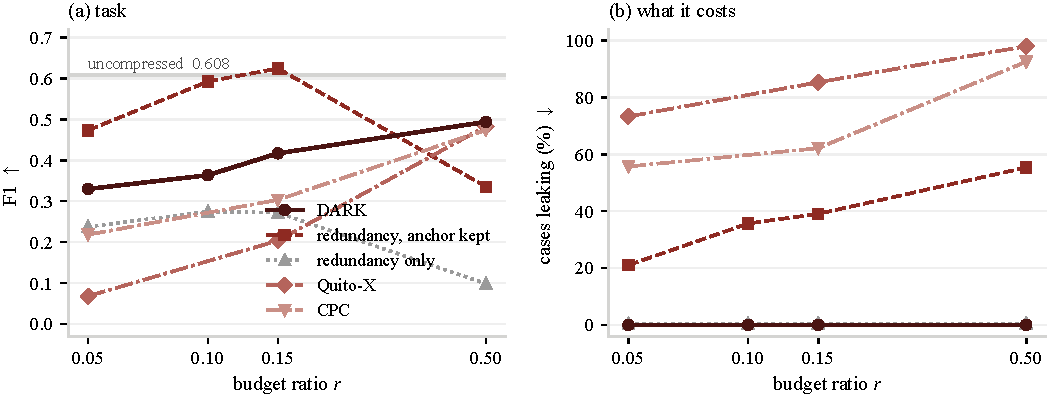
\includegraphics[width=\textwidth]{figures/fig_budget_all.pdf}
\caption{The price of the property, and who pays it. (a)~F1 against the budget ratio;
(b)~the share of cases in which a protected value is recoverable from the prompt, on the same arms
and the same ratios. The internal arms are measured on all $2{,}728$ cases; the two published
compressors on $341$ paired cases at the two tight ratios and on all $2{,}728$ at $r=0.50$.
\textsc{DARK} rises with the budget and stays at $0\%$ throughout. The anchor-kept redundancy arm
overtakes it below $r\approx0.10$ and pays for that with leakage that grows from $21\%$ to $55\%$;
the published compressors do not overtake it at all below $r=0.10$, falling to $0.0679$ and
$0.2181$ while leaking on $73\%$ and $56\%$ of cases. Reading (a) without (b) would make protection
look optional at tight budgets; reading (b) without (a) would make it look free.}
\label{fig:budgetall}
\end{figure*}
